% Options for packages loaded elsewhere
\PassOptionsToPackage{unicode}{hyperref}
\PassOptionsToPackage{hyphens}{url}
\documentclass[
]{article}
\usepackage{xcolor}
\usepackage[margin=1in]{geometry}
\usepackage{amsmath,amssymb}
\setcounter{secnumdepth}{-\maxdimen} % remove section numbering
\usepackage{iftex}
\ifPDFTeX
  \usepackage[T1]{fontenc}
  \usepackage[utf8]{inputenc}
  \usepackage{textcomp} % provide euro and other symbols
\else % if luatex or xetex
  \usepackage{unicode-math} % this also loads fontspec
  \defaultfontfeatures{Scale=MatchLowercase}
  \defaultfontfeatures[\rmfamily]{Ligatures=TeX,Scale=1}
\fi
\usepackage{lmodern}
\ifPDFTeX\else
  % xetex/luatex font selection
\fi
% Use upquote if available, for straight quotes in verbatim environments
\IfFileExists{upquote.sty}{\usepackage{upquote}}{}
\IfFileExists{microtype.sty}{% use microtype if available
  \usepackage[]{microtype}
  \UseMicrotypeSet[protrusion]{basicmath} % disable protrusion for tt fonts
}{}
\makeatletter
\@ifundefined{KOMAClassName}{% if non-KOMA class
  \IfFileExists{parskip.sty}{%
    \usepackage{parskip}
  }{% else
    \setlength{\parindent}{0pt}
    \setlength{\parskip}{6pt plus 2pt minus 1pt}}
}{% if KOMA class
  \KOMAoptions{parskip=half}}
\makeatother
\usepackage{longtable,booktabs,array}
\newcounter{none} % for unnumbered tables
\usepackage{calc} % for calculating minipage widths
% Correct order of tables after \paragraph or \subparagraph
\usepackage{etoolbox}
\makeatletter
\patchcmd\longtable{\par}{\if@noskipsec\mbox{}\fi\par}{}{}
\makeatother
% Allow footnotes in longtable head/foot
\IfFileExists{footnotehyper.sty}{\usepackage{footnotehyper}}{\usepackage{footnote}}
\makesavenoteenv{longtable}
\usepackage{graphicx}
\makeatletter
\newsavebox\pandoc@box
\newcommand*\pandocbounded[1]{% scales image to fit in text height/width
  \sbox\pandoc@box{#1}%
  \Gscale@div\@tempa{\textheight}{\dimexpr\ht\pandoc@box+\dp\pandoc@box\relax}%
  \Gscale@div\@tempb{\linewidth}{\wd\pandoc@box}%
  \ifdim\@tempb\p@<\@tempa\p@\let\@tempa\@tempb\fi% select the smaller of both
  \ifdim\@tempa\p@<\p@\scalebox{\@tempa}{\usebox\pandoc@box}%
  \else\usebox{\pandoc@box}%
  \fi%
}
% Set default figure placement to htbp
\def\fps@figure{htbp}
\makeatother
\setlength{\emergencystretch}{3em} % prevent overfull lines
\providecommand{\tightlist}{%
  \setlength{\itemsep}{0pt}\setlength{\parskip}{0pt}}
\usepackage{bookmark}
\IfFileExists{xurl.sty}{\usepackage{xurl}}{} % add URL line breaks if available
\urlstyle{same}
\hypersetup{
  hidelinks,
  pdfcreator={LaTeX via pandoc}}

\author{}
\date{\vspace{-2.5em}}

\begin{document}

\section{HALLAZGOS --- ENE INE Chile
2010-2026}\label{hallazgos-ene-ine-chile-2010-2026}

\begin{quote}
\textbf{Proyecto:} Análisis del mercado laboral chileno con microdatos
de la Encuesta Nacional de Empleo (ENE)\\
\textbf{Autor:} Felipe Obregón\\
\textbf{Última actualización:} 2026-06-02
\end{quote}

\begin{center}\rule{0.5\linewidth}{0.5pt}\end{center}

\subsection{1. Resumen del Proyecto}\label{resumen-del-proyecto}

Este proyecto descarga, consolida y analiza la totalidad de los
microdatos públicos de la \textbf{Encuesta Nacional de Empleo (ENE)} del
INE Chile para el período \textbf{2010--2026}, cubriendo 210 archivos
CSV trimestrales (\textasciitilde7.3 GB). El objetivo central es
caracterizar la evolución de las tasas de desocupación, ocupación y
participación laboral a nivel nacional y con foco en la \textbf{Región
de Antofagasta (Región 2)}, desagregando por sexo y grupo de edad.

El análisis abarca cinco épocas metodológicas del cuestionario ENE:

{\def\LTcaptype{none} % do not increment counter
\begin{longtable}[]{@{}
  >{\raggedright\arraybackslash}p{(\linewidth - 4\tabcolsep) * \real{0.1707}}
  >{\raggedright\arraybackslash}p{(\linewidth - 4\tabcolsep) * \real{0.2195}}
  >{\raggedright\arraybackslash}p{(\linewidth - 4\tabcolsep) * \real{0.6098}}@{}}
\toprule\noalign{}
\begin{minipage}[b]{\linewidth}\raggedright
Época
\end{minipage} & \begin{minipage}[b]{\linewidth}\raggedright
Período
\end{minipage} & \begin{minipage}[b]{\linewidth}\raggedright
Característica principal
\end{minipage} \\
\midrule\noalign{}
\endhead
\bottomrule\noalign{}
\endlastfoot
1 & 2010--2012 & ENE clásica (CIUO-88, CIIU Rev.3) \\
2 & 2013--2016 & Incorporación rama CAENES \\
3 & 2017--2019 & Nueva ENE (CIUO-08, nuevo marco muestral) \\
4 & 2020--feb/2022 & Cuestionario COVID (migración, plataformas,
turnos) \\
5 & mar/2022--2026 & Estructura estable actual \\
\end{longtable}
}

Los quiebres metodológicos entre épocas (especialmente la transición
2016→2017) deben considerarse al interpretar tendencias de largo plazo.

\begin{center}\rule{0.5\linewidth}{0.5pt}\end{center}

\subsection{2. Descripción de Scripts}\label{descripciuxf3n-de-scripts}

\subsubsection{Scripts Python --- Descarga y
exploración}\label{scripts-python-descarga-y-exploraciuxf3n}

{\def\LTcaptype{none} % do not increment counter
\begin{longtable}[]{@{}
  >{\raggedright\arraybackslash}p{(\linewidth - 2\tabcolsep) * \real{0.4211}}
  >{\raggedright\arraybackslash}p{(\linewidth - 2\tabcolsep) * \real{0.5789}}@{}}
\toprule\noalign{}
\begin{minipage}[b]{\linewidth}\raggedright
Script
\end{minipage} & \begin{minipage}[b]{\linewidth}\raggedright
Propósito
\end{minipage} \\
\midrule\noalign{}
\endhead
\bottomrule\noalign{}
\endlastfoot
\texttt{investigar\_ine.py} & Exploración inicial del sitio INE: detecta
la estructura de URLs, formatos disponibles y nomenclatura de archivos.
Genera \texttt{pagina\_principal.html} como respaldo. \\
\texttt{descargar\_ene.py} & Primera versión del descargador: itera
sobre el catálogo del sitio INE y descarga archivos CSV individualmente
con reintentos básicos. \\
\texttt{descargar\_ene\_v2.py} & Versión mejorada: descarga el
manifiesto completo (\texttt{manifest\_completo.json}, 1.270 entradas),
valida URLs y gestiona errores de red de forma robusta. \\
\texttt{descarga\_csv.py} & Script de producción: descarga masiva de
todos los CSV organizados por año en carpetas \texttt{2010/},
\texttt{2011/}, \ldots, \texttt{2026/}. Implementa control de archivos
ya descargados para reanudar descargas interrumpidas. \\
\end{longtable}
}

\subsubsection{Scripts R --- Consolidación y
análisis}\label{scripts-r-consolidaciuxf3n-y-anuxe1lisis}

{\def\LTcaptype{none} % do not increment counter
\begin{longtable}[]{@{}
  >{\raggedright\arraybackslash}p{(\linewidth - 2\tabcolsep) * \real{0.4211}}
  >{\raggedright\arraybackslash}p{(\linewidth - 2\tabcolsep) * \real{0.5789}}@{}}
\toprule\noalign{}
\begin{minipage}[b]{\linewidth}\raggedright
Script
\end{minipage} & \begin{minipage}[b]{\linewidth}\raggedright
Propósito
\end{minipage} \\
\midrule\noalign{}
\endhead
\bottomrule\noalign{}
\endlastfoot
\texttt{01\_consolidar.R} & Lee los 210 archivos trimestrales, extrae
las variables comparables entre épocas (\texttt{region}, \texttt{sexo},
\texttt{edad}, \texttt{activ}, \texttt{fact\_cal}), y genera el archivo
consolidado \texttt{ene\_consolidado.rds} (\textasciitilde152 MB).
Maneja automáticamente variables ausentes según época. \\
\texttt{02\_eda.R} & Análisis exploratorio principal: calcula tasas
nacionales (desocupación, ocupación, participación) por trimestre,
genera los gráficos 01--03, y exporta
\texttt{resultados/tabla\_resumen\_anual.csv} con tasas anuales
nacionales y de Antofagasta. \\
\texttt{03\_sexo\_edad.R} & Análisis desagregado: tasas por sexo (con
brecha de género), grupos de edad simplificados (15-24 / 25-54 / 55+),
zoom al período COVID y comparación Antofagasta. Genera los gráficos
04--07 y \texttt{resultados/tabla\_sexo\_anual.csv}. \\
\end{longtable}
}

\begin{center}\rule{0.5\linewidth}{0.5pt}\end{center}

\subsection{3. Tabla de Hallazgos Principales por
Año}\label{tabla-de-hallazgos-principales-por-auxf1o}

\subsubsection{3.1 Tasas nacionales y de
Antofagasta}\label{tasas-nacionales-y-de-antofagasta}

{\def\LTcaptype{none} % do not increment counter
\begin{longtable}[]{@{}
  >{\raggedright\arraybackslash}p{(\linewidth - 10\tabcolsep) * \real{0.0532}}
  >{\centering\arraybackslash}p{(\linewidth - 10\tabcolsep) * \real{0.1702}}
  >{\centering\arraybackslash}p{(\linewidth - 10\tabcolsep) * \real{0.1702}}
  >{\centering\arraybackslash}p{(\linewidth - 10\tabcolsep) * \real{0.1702}}
  >{\centering\arraybackslash}p{(\linewidth - 10\tabcolsep) * \real{0.2021}}
  >{\centering\arraybackslash}p{(\linewidth - 10\tabcolsep) * \real{0.2340}}@{}}
\toprule\noalign{}
\begin{minipage}[b]{\linewidth}\raggedright
Año
\end{minipage} & \begin{minipage}[b]{\linewidth}\centering
TD Nacional (\%)
\end{minipage} & \begin{minipage}[b]{\linewidth}\centering
TO Nacional (\%)
\end{minipage} & \begin{minipage}[b]{\linewidth}\centering
TP Nacional (\%)
\end{minipage} & \begin{minipage}[b]{\linewidth}\centering
TD Antofagasta (\%)
\end{minipage} & \begin{minipage}[b]{\linewidth}\centering
Brecha Antof−Nac (pp)
\end{minipage} \\
\midrule\noalign{}
\endhead
\bottomrule\noalign{}
\endlastfoot
2010 & 8.22 & 55.21 & 60.16 & 7.56 & −0.66 \\
2011 & 7.32 & 56.97 & 61.47 & 6.27 & −1.05 \\
2012 & 6.58 & 57.43 & 61.48 & 5.30 & −1.28 \\
2013 & 6.13 & 57.82 & 61.60 & 5.94 & −0.19 \\
2014 & 6.42 & 57.90 & 61.87 & 6.62 & +0.20 \\
2015 & 6.37 & 58.06 & 62.01 & 6.77 & +0.40 \\
2016 & 6.68 & 58.00 & 62.15 & 8.15 & +1.47 \\
2017 & 6.97 & 58.32 & 62.69 & 8.66 & +1.69 \\
2018 & 7.36 & 58.35 & 62.98 & 8.71 & +1.35 \\
2019 & 7.24 & 58.27 & 62.82 & 8.02 & +0.78 \\
\textbf{2020} & \textbf{10.70} & \textbf{49.98} & \textbf{55.97} &
\textbf{11.32} & \textbf{+0.62} \\
2021 & 8.85 & 52.15 & 57.21 & 9.53 & +0.68 \\
2022 & 7.85 & 55.03 & 59.71 & 8.14 & +0.29 \\
2023 & 8.67 & 55.87 & 61.17 & 8.19 & −0.48 \\
2024 & 8.47 & 56.74 & 61.99 & 8.36 & −0.11 \\
2025 & 8.56 & 56.76 & 62.08 & 6.84 & −1.72 \\
2026* & 8.79 & 56.84 & 62.32 & 6.74 & −2.05 \\
\end{longtable}
}

*2026: datos parciales (enero--marzo).\\
\textbf{TD} = Tasa de desocupación · \textbf{TO} = Tasa de ocupación ·
\textbf{TP} = Tasa de participación.

\subsubsection{3.2 Brecha de género en la tasa de desocupación (Mujer −
Hombre,
pp)}\label{brecha-de-guxe9nero-en-la-tasa-de-desocupaciuxf3n-mujer-hombre-pp}

{\def\LTcaptype{none} % do not increment counter
\begin{longtable}[]{@{}
  >{\raggedright\arraybackslash}p{(\linewidth - 8\tabcolsep) * \real{0.0641}}
  >{\centering\arraybackslash}p{(\linewidth - 8\tabcolsep) * \real{0.2436}}
  >{\centering\arraybackslash}p{(\linewidth - 8\tabcolsep) * \real{0.2308}}
  >{\centering\arraybackslash}p{(\linewidth - 8\tabcolsep) * \real{0.2179}}
  >{\centering\arraybackslash}p{(\linewidth - 8\tabcolsep) * \real{0.2436}}@{}}
\toprule\noalign{}
\begin{minipage}[b]{\linewidth}\raggedright
Año
\end{minipage} & \begin{minipage}[b]{\linewidth}\centering
TD Hombre Nac (\%)
\end{minipage} & \begin{minipage}[b]{\linewidth}\centering
TD Mujer Nac (\%)
\end{minipage} & \begin{minipage}[b]{\linewidth}\centering
Brecha Nac (pp)
\end{minipage} & \begin{minipage}[b]{\linewidth}\centering
Brecha Antof (pp)
\end{minipage} \\
\midrule\noalign{}
\endhead
\bottomrule\noalign{}
\endlastfoot
2010 & 7.18 & 9.80 & +2.62 & +1.16 \\
2012 & 5.56 & 8.06 & +2.50 & +1.80 \\
2014 & 6.02 & 6.98 & +0.96 & +0.26 \\
2016 & 6.30 & 7.22 & +0.92 & −0.12 \\
2018 & 6.75 & 8.18 & +1.43 & +1.66 \\
2019 & 6.66 & 8.03 & +1.37 & +2.56 \\
2020 & 10.54 & 10.94 & +0.40 & −0.38 \\
2021 & 8.63 & 9.16 & +0.53 & −1.22 \\
2023 & 8.35 & 9.10 & +0.75 & +0.04 \\
2025 & 8.02 & 9.28 & +1.26 & +1.71 \\
2026* & 7.99 & 9.82 & +1.83 & +2.83 \\
\end{longtable}
}

\begin{center}\rule{0.5\linewidth}{0.5pt}\end{center}

\subsection{4. Interpretación de
Gráficos}\label{interpretaciuxf3n-de-gruxe1ficos}

\#\#\textbf{Tasa de desocupación nacional por sexo, 2010--2026 (con
LOESS y hitos)}

\#\pandocbounded{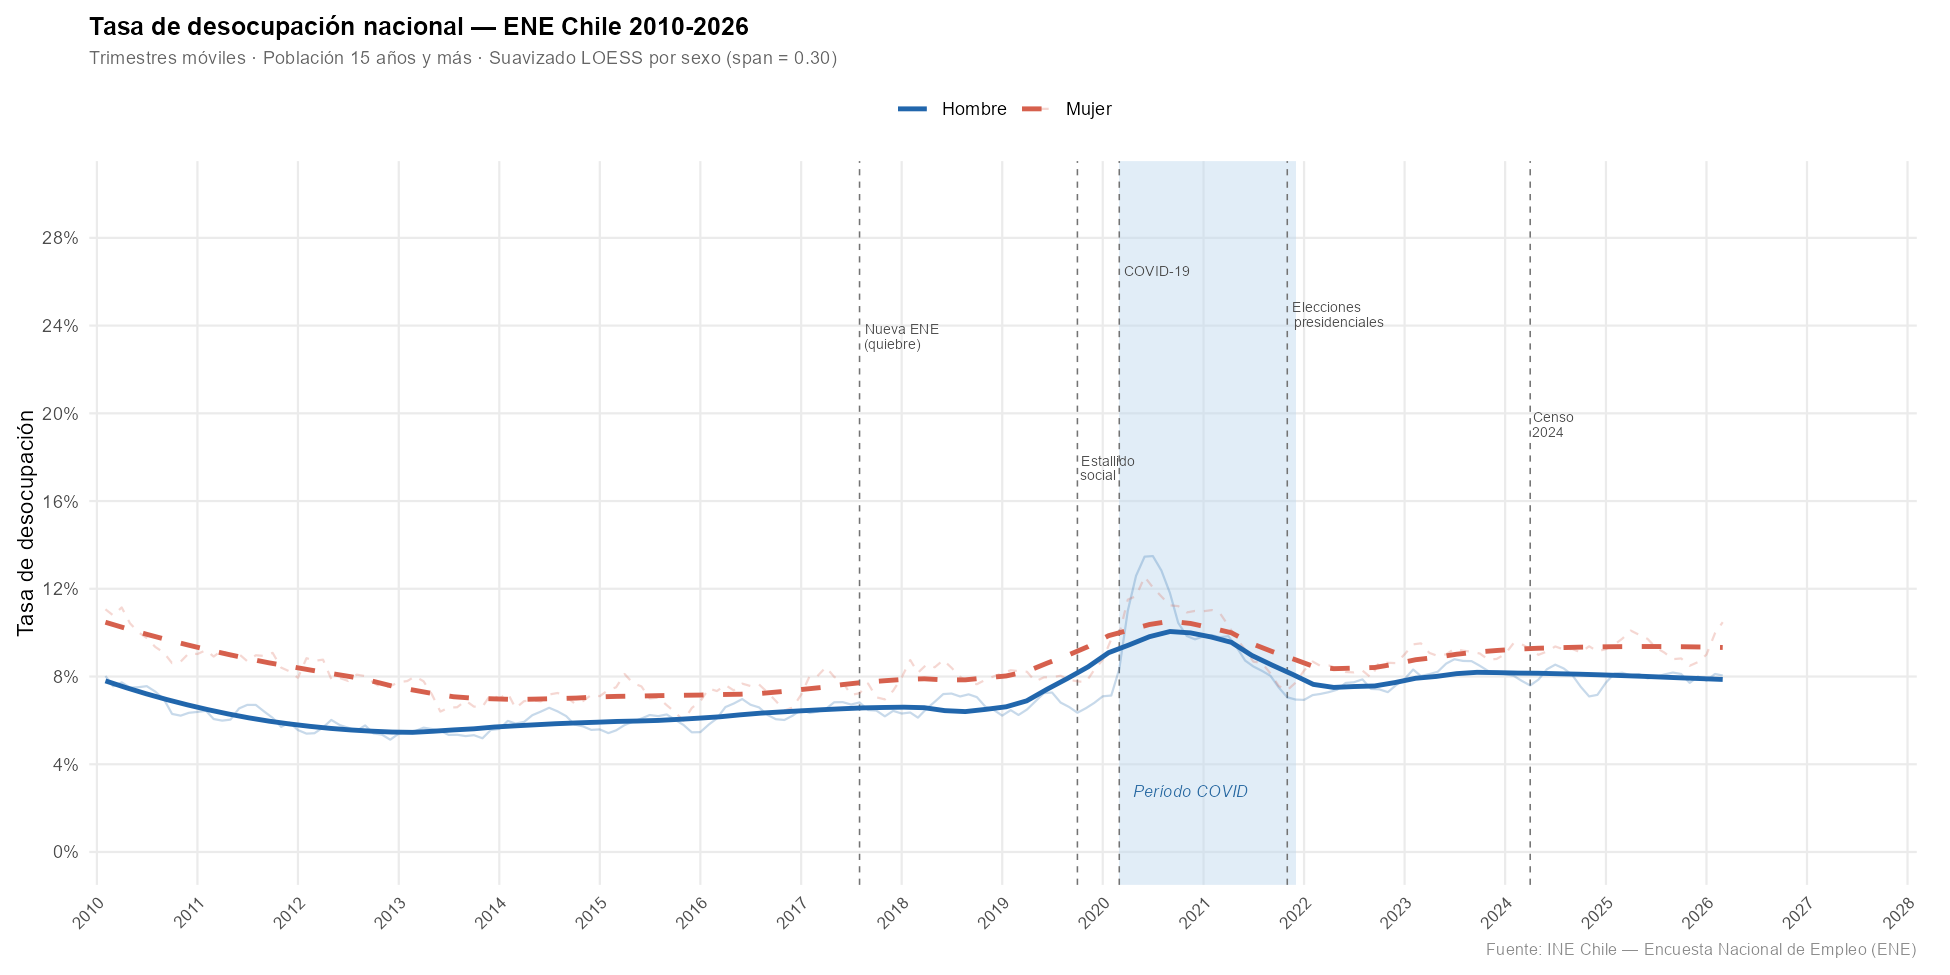
\includegraphics[keepaspectratio,alt={Desocupacion nacional(Gráfico 1)}]{graficos/01_desocupacion_nacional.png}}

\begin{itemize}
\tightlist
\item
  La desocupación femenina se mantuvo consistentemente por encima de la
  masculina durante toda la serie, con una brecha media de
  \textasciitilde1.5 pp en el período pre-COVID.
\item
  Se observa una \textbf{tendencia descendente} desde el pico
  post-crisis de 2010 (8.2\%) hasta el mínimo de 2013 (6.1\%), seguida
  de una leve alza hacia 2018--2019.
\item
  La \textbf{Nueva ENE (2017)} produce un quiebre metodológico visible:
  la serie mujer presenta un salto ascendente que parcialmente refleja
  el cambio de marco muestral y no necesariamente deterioro real del
  mercado.
\item
  El \textbf{Estallido Social (oct-2019)} anticipa una ligera presión al
  alza antes del shock COVID.
\item
  El \textbf{período COVID (2020--2021)} es el evento más disruptivo: la
  TD nacional sube de \textasciitilde7\% a un máximo de
  \textasciitilde14\% (trimestres móviles), con posterior recuperación
  hacia 2022--2023. La brecha de género se comprimió durante COVID
  porque la desocupación masculina subió más abruptamente.
\item
  En 2023--2026 la desocupación se estabiliza en torno al 8.5--9\%, por
  encima del nivel pre-COVID, sin señal clara de convergencia hacia los
  mínimos de 2012--2013.
\end{itemize}

\begin{center}\rule{0.5\linewidth}{0.5pt}\end{center}

\#\#\textbf{Tasa de desocupación por grupo etario (6 grupos),
2010--2026}

\begin{figure}
\centering
\pandocbounded{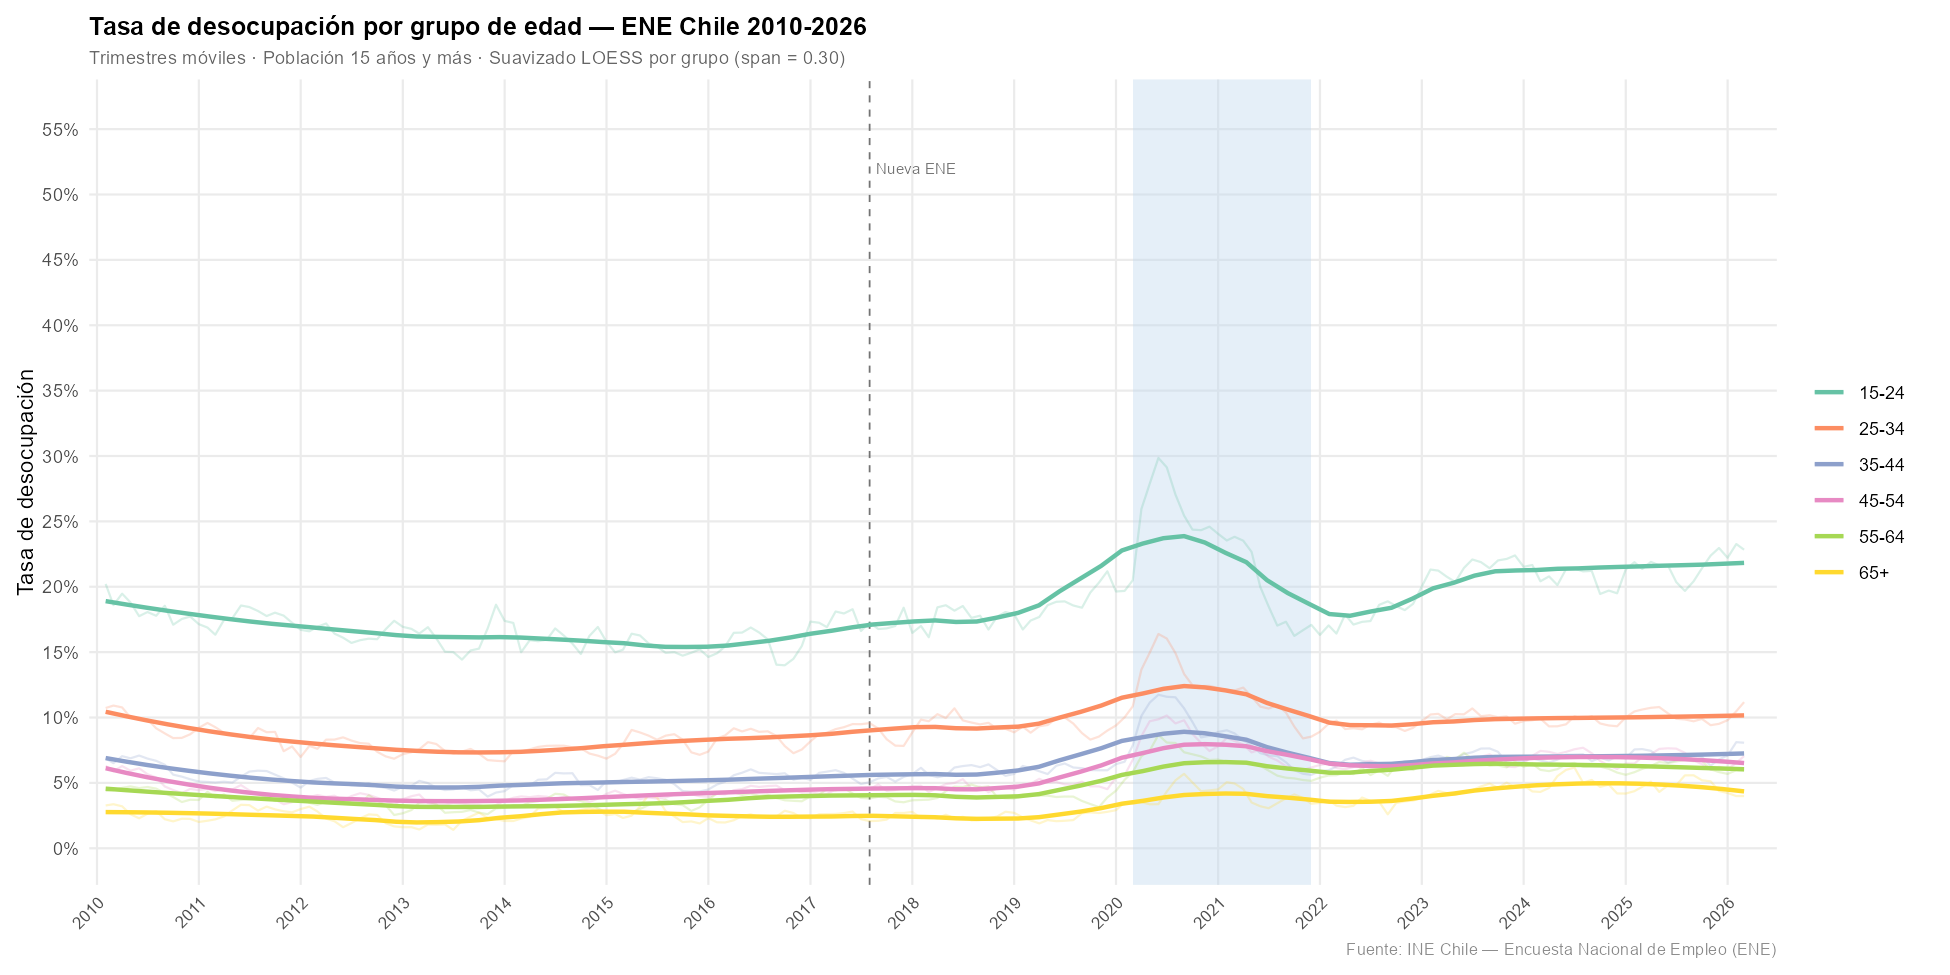
\includegraphics[keepaspectratio,alt={Desocupación por Edad (Gráfico 2)}]{graficos/02_desocupacion_edad.png}}
\caption{Desocupación por Edad (Gráfico 2)}
\end{figure}

\begin{itemize}
\tightlist
\item
  El grupo \textbf{15--24 años} (desocupación juvenil) es el de mayor
  volatilidad y nivel, oscilando entre el 15\% y el 50\% según
  trimestre. El pico COVID superó el 30\% en tendencia LOESS.
\item
  Los grupos \textbf{25--34} y \textbf{35--44} presentan niveles
  intermedios y son los más afectados en términos absolutos de personas
  dado su tamaño.
\item
  Los grupos de \textbf{55+ y 65+} exhiben las tasas más bajas y menor
  sensibilidad cíclica, coherente con mayor selectividad en la búsqueda
  de empleo y menor participación laboral.
\item
  El quiebre de la \textbf{Nueva ENE (2017)} es especialmente
  pronunciado en el grupo 15--24, cuya tasa experimenta un salto
  discontinuo que debe interpretarse con cautela metodológica.
\item
  La recuperación post-COVID fue más lenta en los jóvenes: en 2023--2026
  su tasa se mantiene \textasciitilde5 pp por encima del nivel previo al
  COVID.
\end{itemize}

\begin{center}\rule{0.5\linewidth}{0.5pt}\end{center}

\#\#\textbf{Antofagasta (Región 2) vs.~Nacional, 2010--2026}

\begin{figure}
\centering
\pandocbounded{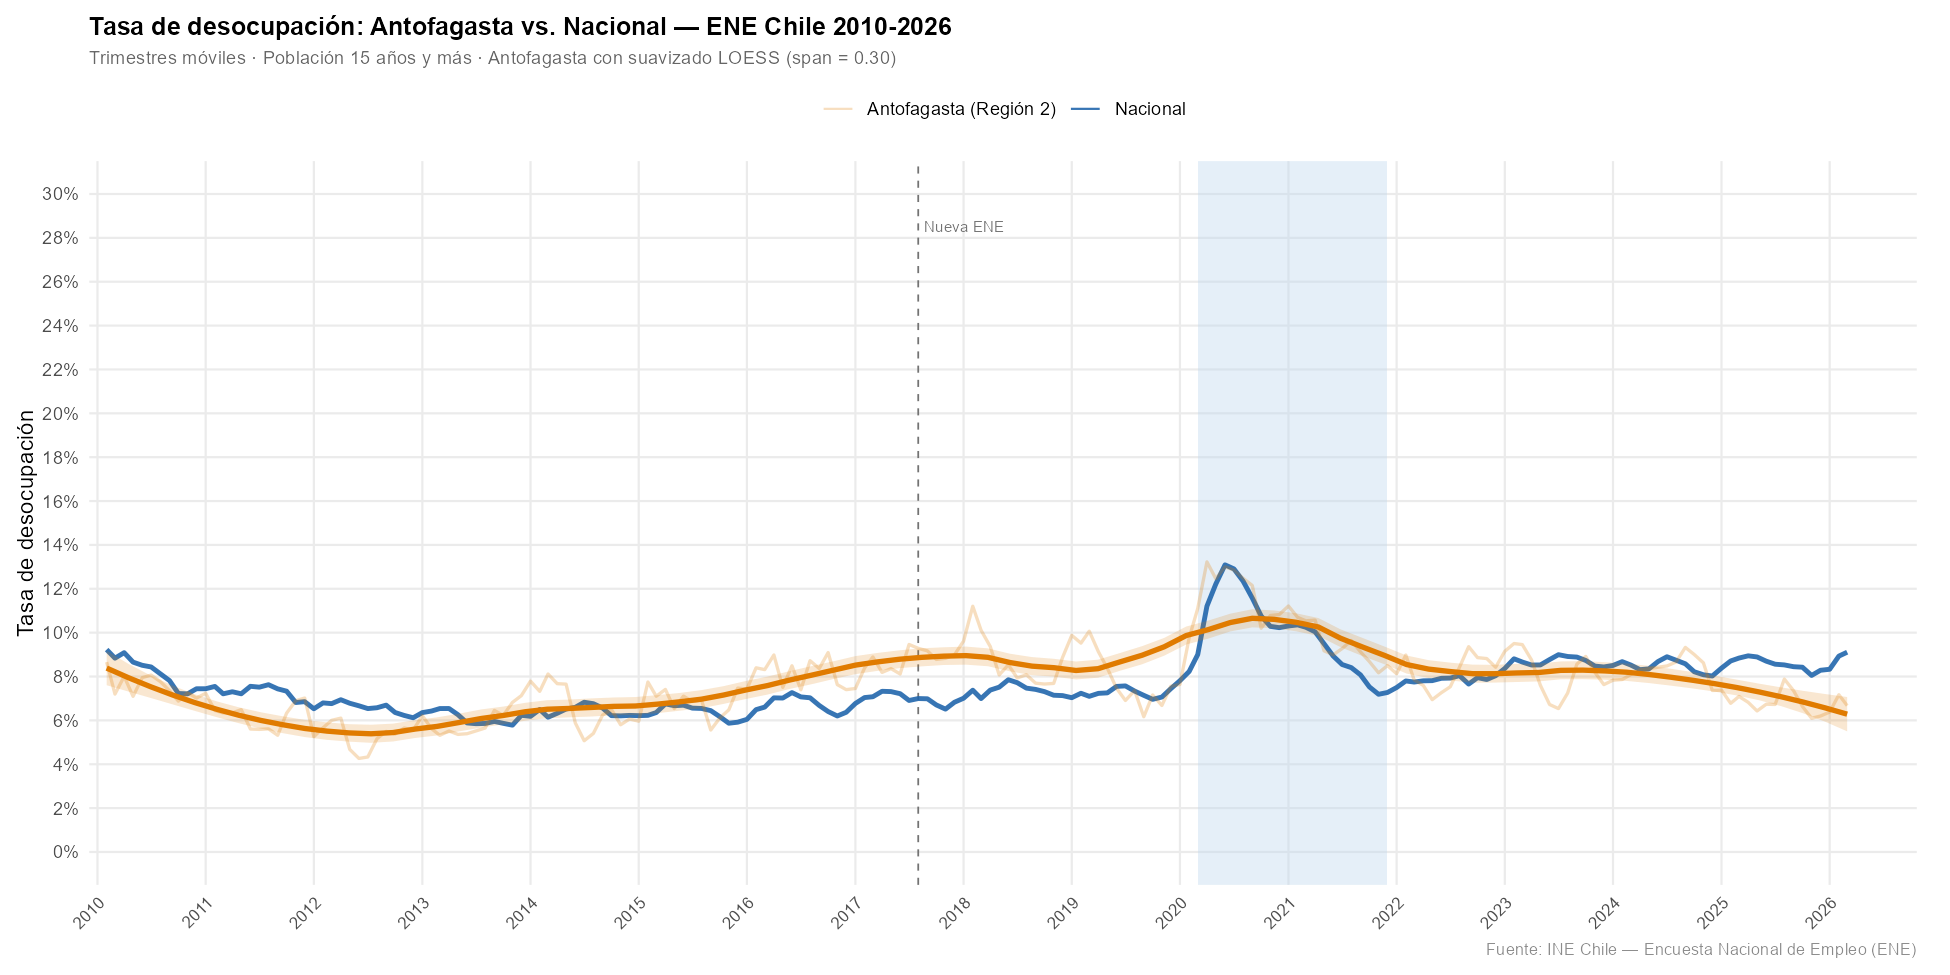
\includegraphics[keepaspectratio,alt={Antofagasta vs nacional (Gráfico 3)}]{graficos/03_antofagasta_vs_nacional.png}}
\caption{Antofagasta vs nacional (Gráfico 3)}
\end{figure}

\begin{itemize}
\tightlist
\item
  Hasta 2013, Antofagasta tenía una TD \textbf{inferior} a la nacional
  en \textasciitilde1 pp, posiblemente por el auge minero y la alta
  demanda de empleo.
\item
  A partir de 2014--2015 la situación se \textbf{invierte}: la región
  supera al promedio nacional y la brecha se amplía hasta
  \textasciitilde1.7 pp en 2017--2018, coincidiendo con la
  desaceleración del ciclo minero del cobre.
\item
  Durante COVID, Antofagasta registró la misma magnitud de shock que el
  nivel nacional (+0.62 pp de brecha), pero con mayor volatilidad
  trimestral dada la menor muestra regional.
\item
  El rasgo más destacado del período reciente (2023--2026) es que
  \textbf{Antofagasta volvió a situarse por debajo de la media
  nacional}, con una brecha negativa que alcanzó −2.05 pp en 2026
  (enero--marzo). Esto sugiere una recuperación liderada por el sector
  minero post-pandemia.
\end{itemize}

\begin{center}\rule{0.5\linewidth}{0.5pt}\end{center}

\#\#\textbf{Brecha de género nacional (TD y panel de brecha),
2010--2026}

\begin{figure}
\centering
\pandocbounded{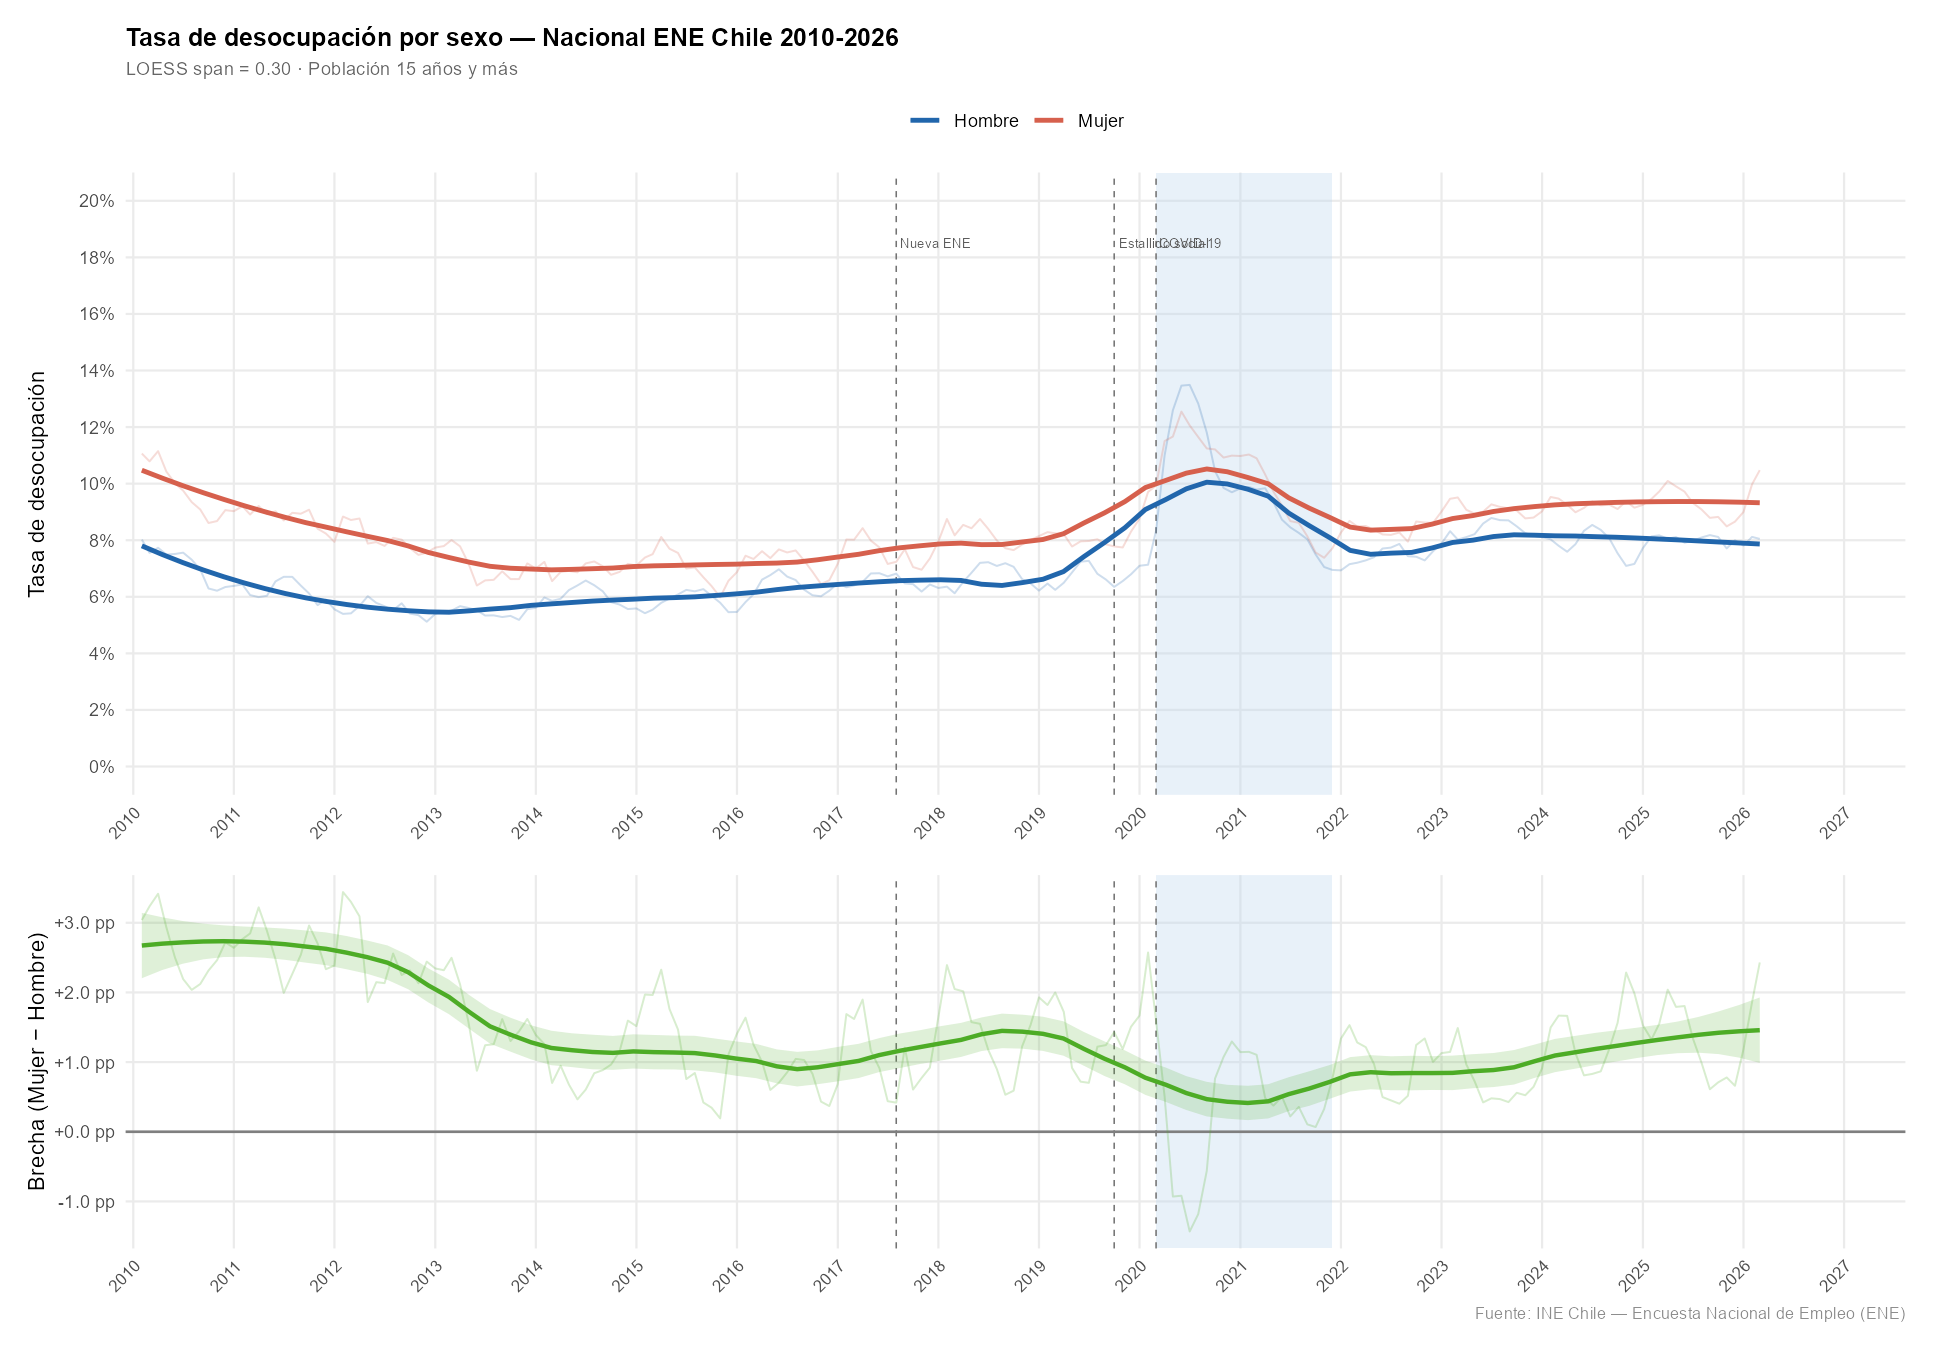
\includegraphics[keepaspectratio,alt={Brecha de género naciona (Gráfico 4)}]{graficos/04_desocupacion_sexo_nacional.png}}
\caption{Brecha de género naciona (Gráfico 4)}
\end{figure}

\begin{itemize}
\tightlist
\item
  El panel superior confirma la persistencia histórica de la brecha: la
  TD femenina supera en promedio 1.5--2.5 pp a la masculina en el
  período 2010--2019.
\item
  El panel inferior (brecha Mujer − Hombre) muestra que la brecha se
  \textbf{comprimió marcadamente durante COVID} (llegando a
  \textasciitilde0.4 pp), porque el mercado laboral masculino es más
  sensible a las contracciones económicas, especialmente en sectores
  como construcción y transporte.
\item
  Tras COVID, la brecha se recuperó hacia los valores históricos: en
  2025--2026 alcanza 1.26--1.83 pp, con tendencia al alza que podría
  indicar mayor dificultad de reinserción femenina post-pandemia.
\end{itemize}

\begin{center}\rule{0.5\linewidth}{0.5pt}\end{center}

\#\#\textbf{Brecha de género en Antofagasta (TD y panel de brecha),
2010--2026}

\begin{figure}
\centering
\pandocbounded{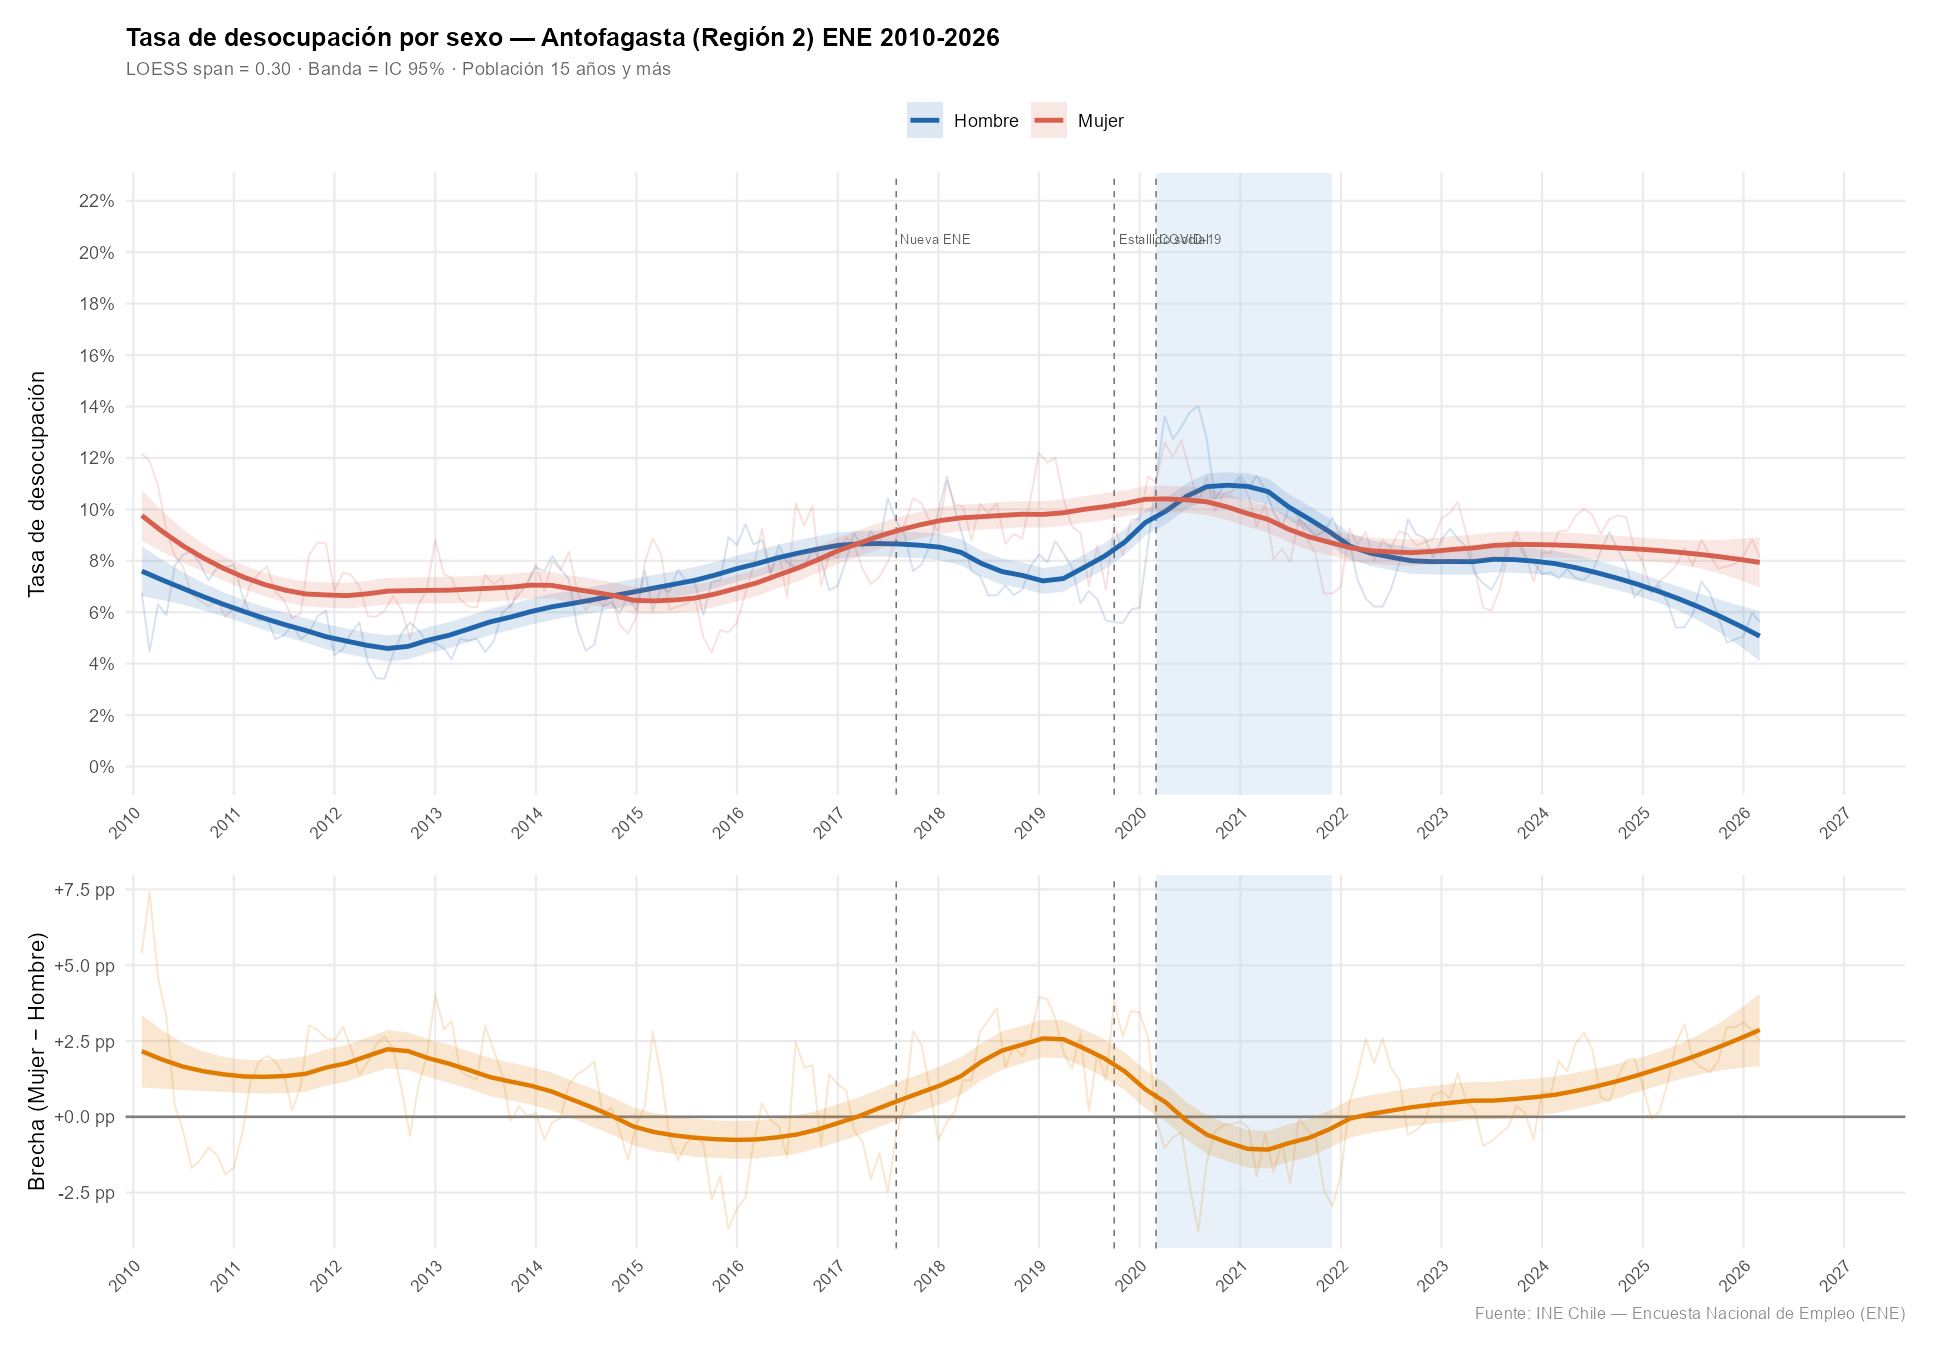
\includegraphics[keepaspectratio,alt={Desocupacion sexo antofagasta (Gráfico 5)}]{graficos/05_desocupacion_sexo_antofagasta.png}}
\caption{Desocupacion sexo antofagasta (Gráfico 5)}
\end{figure}

\begin{itemize}
\tightlist
\item
  Antofagasta muestra una estructura de género atípica: en varios
  períodos (2015--2016, 2020--2021) la brecha se \textbf{invierte}, es
  decir, los hombres tienen mayor TD que las mujeres. Esto refleja el
  carácter masculinizado del sector minero: en fases de contracción, el
  desempleo masculino sube más que el femenino.
\item
  La banda de incertidumbre (IC 95\%) del LOESS es notablemente más
  amplia que en el gráfico nacional, evidenciando la menor precisión de
  las estimaciones regionales por tamaño de muestra.
\item
  En 2019 se observó la mayor brecha en favor de las mujeres (+2.56 pp),
  seguida de una inversión en 2021 (−1.22 pp), lo que marca la asimetría
  sectorial de los shocks en la región.
\item
  En 2026 la brecha vuelve a ser positiva (+2.83 pp), la más alta de
  toda la serie para Antofagasta, señal de que la recuperación minera
  beneficia más al empleo masculino.
\end{itemize}

\begin{center}\rule{0.5\linewidth}{0.5pt}\end{center}

\#\#\textbf{Desocupación juvenil (15-24) vs.~adulta (25-54) y mayores
(55+), 2010--2026}

\begin{figure}
\centering
\pandocbounded{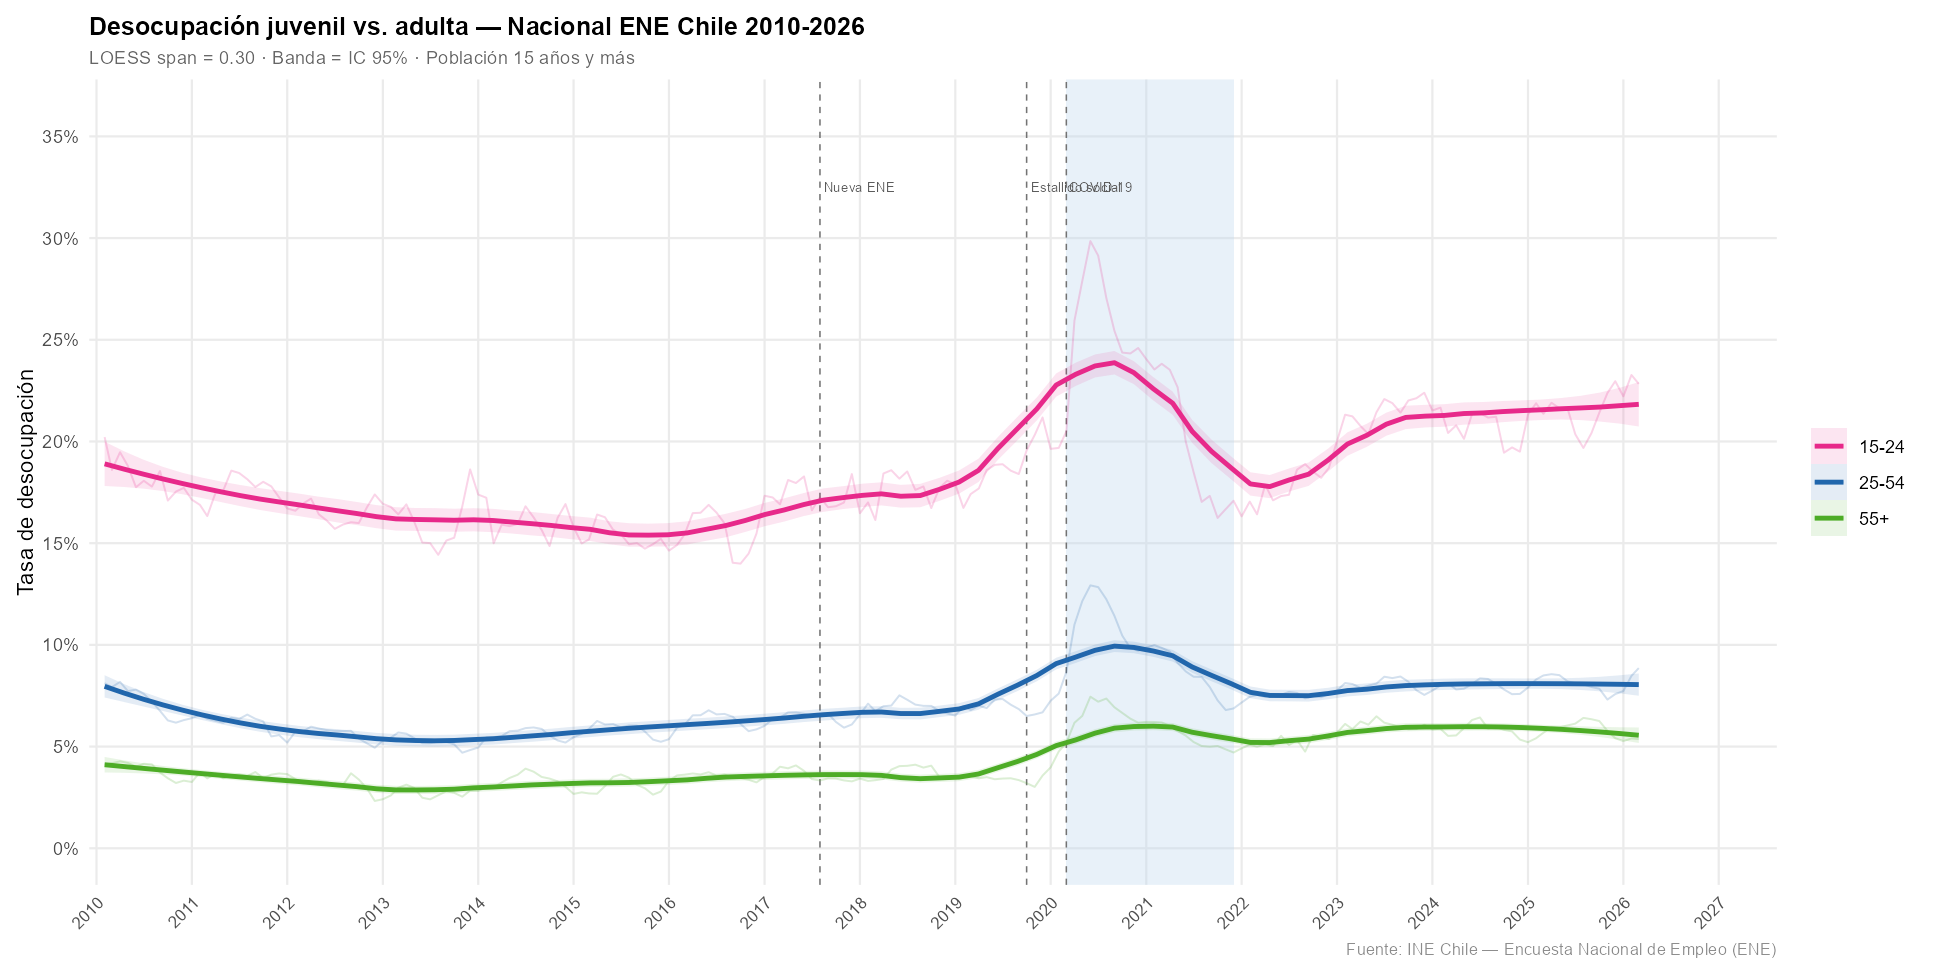
\includegraphics[keepaspectratio,alt={Desocupacion grupos edad (Gráfico 6)}]{graficos/06_desocupacion_grupos_edad.png}}
\caption{Desocupacion grupos edad (Gráfico 6)}
\end{figure}

06\_desocupacion\_grupos\_edad

\begin{itemize}
\tightlist
\item
  La brecha entre desocupación juvenil y adulta es estructuralmente
  grande: el grupo 15--24 duplica o triplica la TD del grupo 25--54 en
  todos los años.
\item
  COVID impactó de forma diferencial: el grupo 25--54 registró el mayor
  salto absoluto en puntos porcentuales (de \textasciitilde5\% a
  \textasciitilde12\%), mientras que en 15--24 el shock fue
  relativamente menor en términos de variación relativa dado su ya
  elevado nivel base.
\item
  El grupo 55+ mostró la mayor resiliencia al COVID, con un pico
  inferior al 10\%, y fue el primero en recuperarse.
\item
  En el período 2023--2026, la desocupación juvenil (15--24) permanece
  por encima del 20\% en la tendencia LOESS, muy por encima del mínimo
  de \textasciitilde15\% registrado en 2012--2013.
\end{itemize}

\begin{center}\rule{0.5\linewidth}{0.5pt}\end{center}

\#\#\textbf{Zoom período COVID (2019--2022): TD y tasa de participación
por sexo}

\begin{figure}
\centering
\pandocbounded{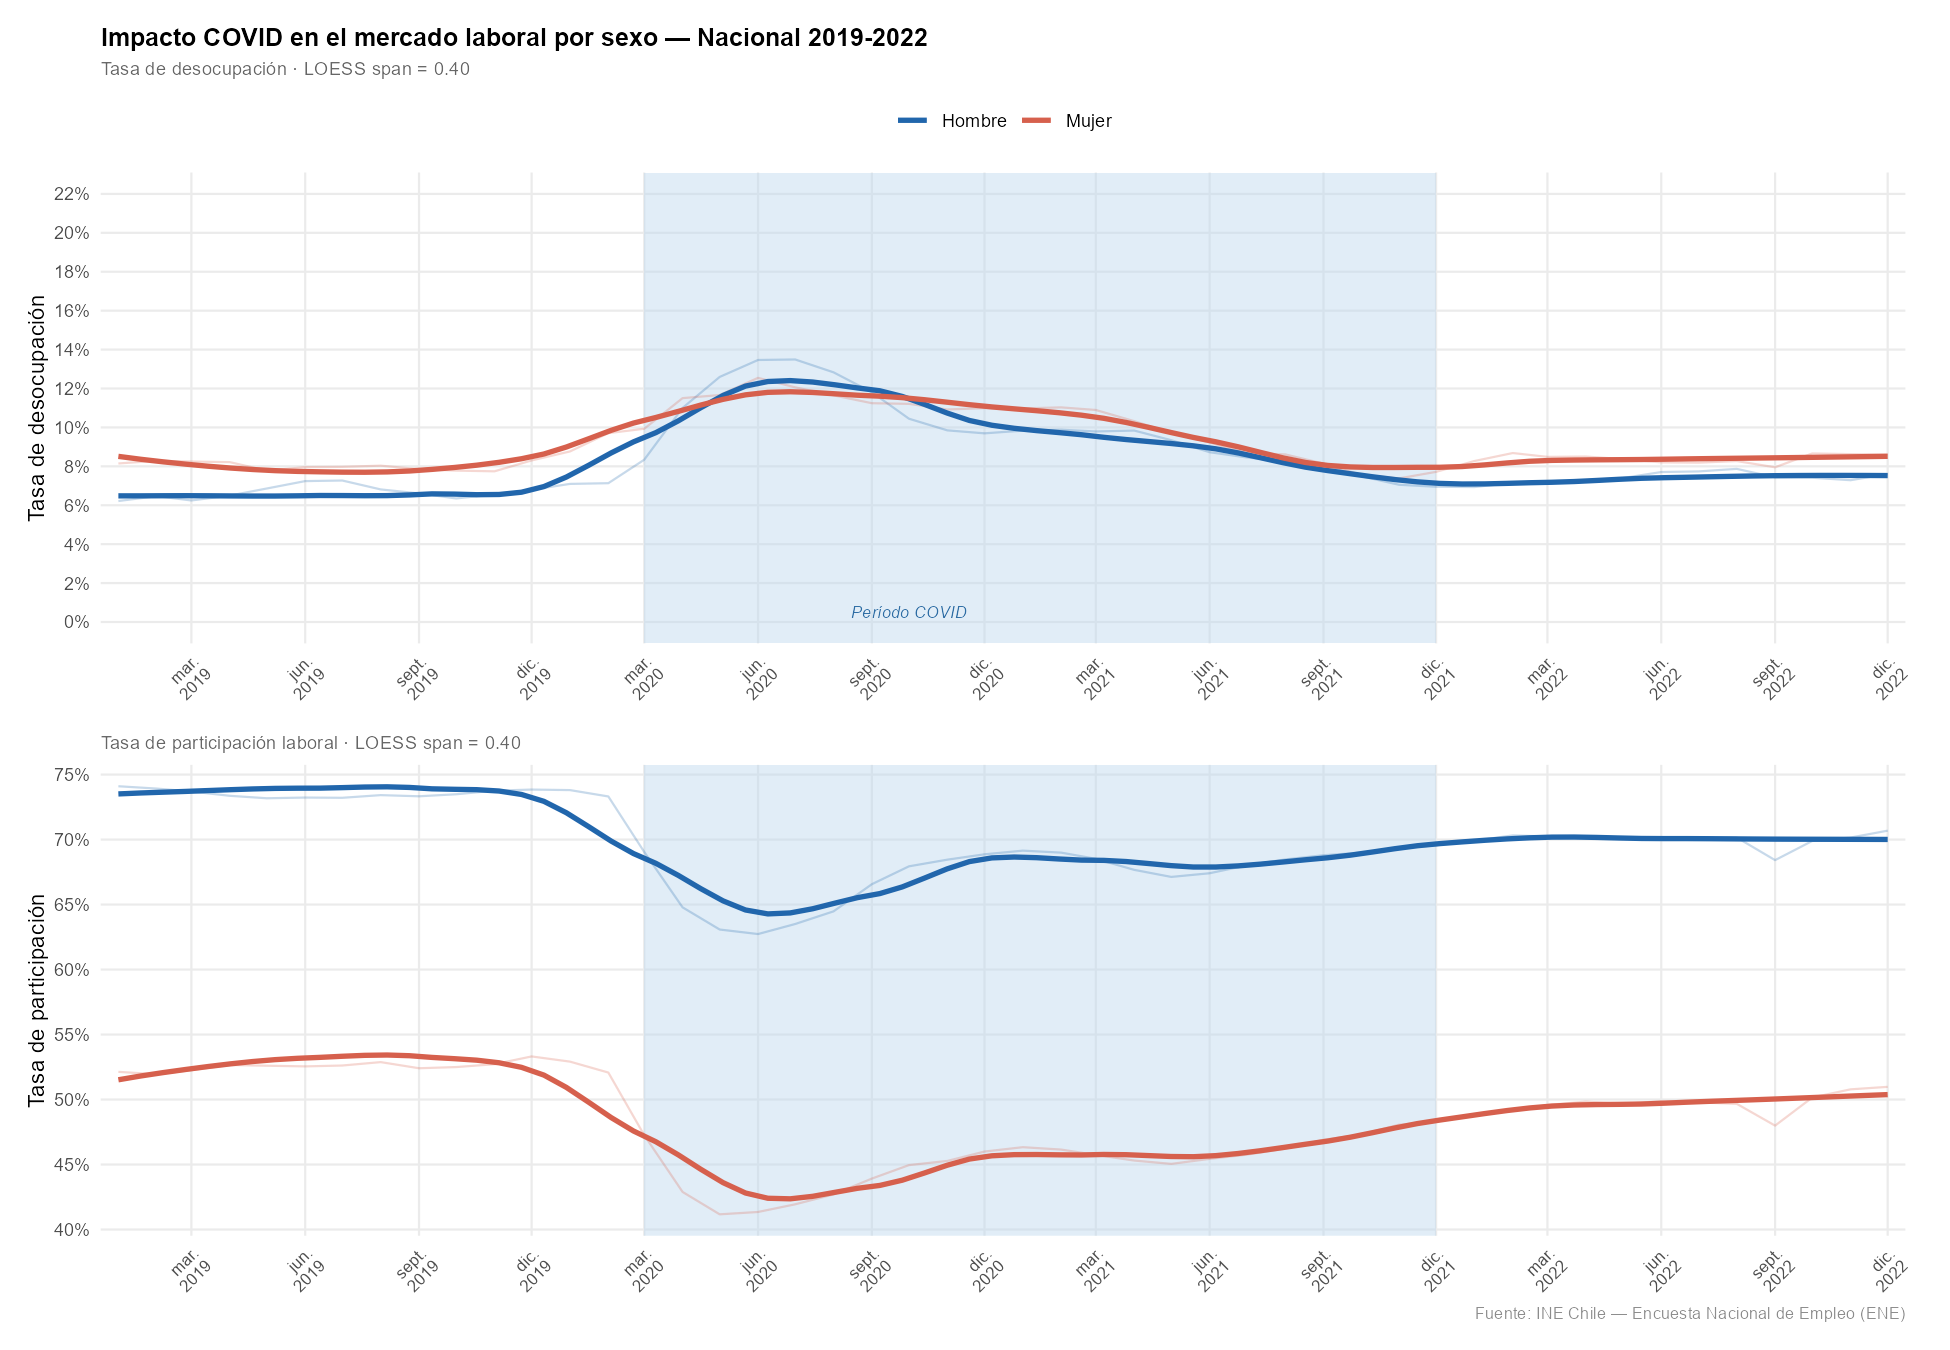
\includegraphics[keepaspectratio,alt={Covid por sexo}]{graficos/07_covid_por_sexo.png}}
\caption{Covid por sexo}
\end{figure}

\begin{itemize}
\tightlist
\item
  El panel superior (TD) muestra el rápido ascenso hacia la desocupación
  máxima en el segundo trimestre de 2020, con ambos sexos alcanzando
  \textasciitilde13--14\% simultáneamente.
\item
  El panel inferior (tasa de participación) es el hallazgo más
  revelador: \textbf{las mujeres registraron una caída de participación
  mucho más pronunciada} (de \textasciitilde48\% a \textasciitilde38\%),
  mientras los hombres cayeron de \textasciitilde70\% a
  \textasciitilde63\%. Esto indica un fenómeno de \textbf{desaliento
  selectivo femenino}: muchas mujeres dejaron de buscar empleo (salen de
  la PEA) en lugar de aparecer como desocupadas.
\item
  La recuperación de la participación femenina fue más lenta y aún en
  2022 no había recuperado completamente el nivel pre-COVID, lo que
  explica por qué la brecha de desocupación se comprimió: el denominador
  (PEA femenina) cayó más que el numerador.
\end{itemize}

\begin{center}\rule{0.5\linewidth}{0.5pt}\end{center}

\subsection{5. Próximos Pasos
Pendientes}\label{pruxf3ximos-pasos-pendientes}

\subsubsection{Análisis estadístico}\label{anuxe1lisis-estaduxedstico}

\begin{itemize}
\tightlist
\item[$\square$]
  \textbf{Modelo de regresión de series de tiempo} (ARIMA o regresión
  con variables dummy de época y eventos) para descomponer tendencia,
  estacionalidad y efectos de hitos (COVID, quiebre 2017, estallido
  social).
\item[$\square$]
  \textbf{Análisis de convergencia regional}: comparar todas las
  regiones para contextualizar la trayectoria de Antofagasta dentro del
  país.
\item[$\square$]
  \textbf{Desagregación por rama de actividad} (variable CAENES,
  disponible desde 2013): cuantificar el peso del sector minero en la
  dinámica de Antofagasta.
\item[$\square$]
  \textbf{Análisis de subempleo y condiciones de empleo} con variables
  adicionales disponibles en las épocas 4 y 5 (trabajo en plataformas,
  trabajo a tiempo parcial involuntario).
\end{itemize}

\subsubsection{Visualización}\label{visualizaciuxf3n}

\begin{itemize}
\tightlist
\item[$\square$]
  \textbf{Mapa choropleth} de tasas regionales por año con \texttt{sf} y
  los límites administrativos de Chile para comunicar heterogeneidad
  geográfica.
\item[$\square$]
  \textbf{Dashboard interactivo} con \texttt{flexdashboard} o Shiny que
  permita explorar la serie por región, grupo de edad y sexo con filtros
  dinámicos.
\item[$\square$]
  \textbf{Gráfico de calor (heatmap) trimestral} con eje x = año, eje y
  = mes, color = TD nacional, para visualizar estacionalidad.
\end{itemize}

\subsubsection{Validación y
reproducibilidad}\label{validaciuxf3n-y-reproducibilidad}

\begin{itemize}
\tightlist
\item[$\square$]
  \textbf{Comparar estimaciones propias con publicaciones oficiales INE}
  (Boletín de Empleo Trimestral) para validar la metodología de
  expansión con \texttt{fact\_cal}.
\item[$\square$]
  \textbf{Documentar el quiebre 2016→2017} con prueba de Chow u otro
  test de cambio estructural para cuantificar su magnitud.
\item[$\square$]
  Empaquetar el pipeline en un \texttt{Makefile} o script
  \texttt{run\_all.R} que ejecute los tres scripts en orden.
\item[$\square$]
  Migrar el \texttt{.rds} a \textbf{formato Parquet} (con
  \texttt{arrow}) para mejorar interoperabilidad con Python/DuckDB.
\end{itemize}

\subsubsection{Comunicación}\label{comunicaciuxf3n}

\begin{itemize}
\tightlist
\item[$\square$]
  Redactar un \textbf{informe ejecutivo de 2 páginas} con los hallazgos
  clave orientado a tomadores de decisiones en política laboral.
\item[$\square$]
  Publicar los resultados en un repositorio GitHub Pages con los
  gráficos embebidos.
\end{itemize}

\begin{center}\rule{0.5\linewidth}{0.5pt}\end{center}

\emph{Fuente: INE Chile --- Encuesta Nacional de Empleo (ENE),
microdatos 2010--2026.}\\
\emph{Metodología: expansión por factor de calibración
\texttt{fact\_cal}. Suavizado LOESS con \texttt{span\ =\ 0.30}. Análisis
realizado en R (data.table, ggplot2).}

\end{document}
